% !TeX root = ..\essay.tex

% Notes from slides

% Erfolg der Methode
% 	Nutzung der Methode in der Literatur
% 	Ergebnisse auf anderen Corpora/Daten
% Literaturrecherche
% 	Erweiterungen der Methode
% 	Kritik der Methode
% Ver-/Anwendung der Methode
% theoretischer Bezug
% Praktischer Bezug
% Verwendbarkeit
% Beschreibung der Methodik
% Bewertung der Methode
% Verwendung von (Fach-)Begriffen richtig und konsistent
% Mit eigenen Worten
% Wissenschaftliches Arbeiten
% Korrekte Zitierweise
% Weiterfuehrende Ideen und Gedanken

% What is the prob­lem that the au­thors tried to solve in this paper?
% How does this prob­lem re­late to the topic of the sem­i­nar and to other talks in the sem­i­nar?
% How can I ex­plain the au­thors' so­lu­tion in the best way?
% How did the au­thors demon­strate that the so­lu­tion works?

\subsection{Step 2 - Creating Hierarchies}

\subsubsection{Introduction}

In the second step of our pipeline, we created tree hierarchies out of the sentences that were selected in the first step. The results of the content selection created a list of sentences for each topic. Our system took those sentences and created a tree with each branching tree indicating a new subtopic. Each node of a tree contained one or more sentences. At the top is a root level with multiple trees that differ in the topics of their sentences. 

The tree hierarchies are built for the third step to better distinguish between topics of sentences. Each resulting tree should contain sentences that are similar in meaning and topic. At the top of each tree should be the most general sentence and at the bottom the most specific sentence.


\subsubsection{Method}

To prepare the Nuggets for the rest of this method we removed stopwords and words with a length lower than three, tokenized the words and we stemmed the words. For a list of stopwords, tokenization and stemming we used NLTK \citep{nltk}.

% TODO https://www.nltk.org/

Our method can be described in three steps. First, we defined a recursive function to insert a sentence into the resulting tree. Then we defined two functions to determinate where to go in the tree. These functions also implement how similarity and specific/general sentences are calculated.

\begin{figure}[H]
	\centering
	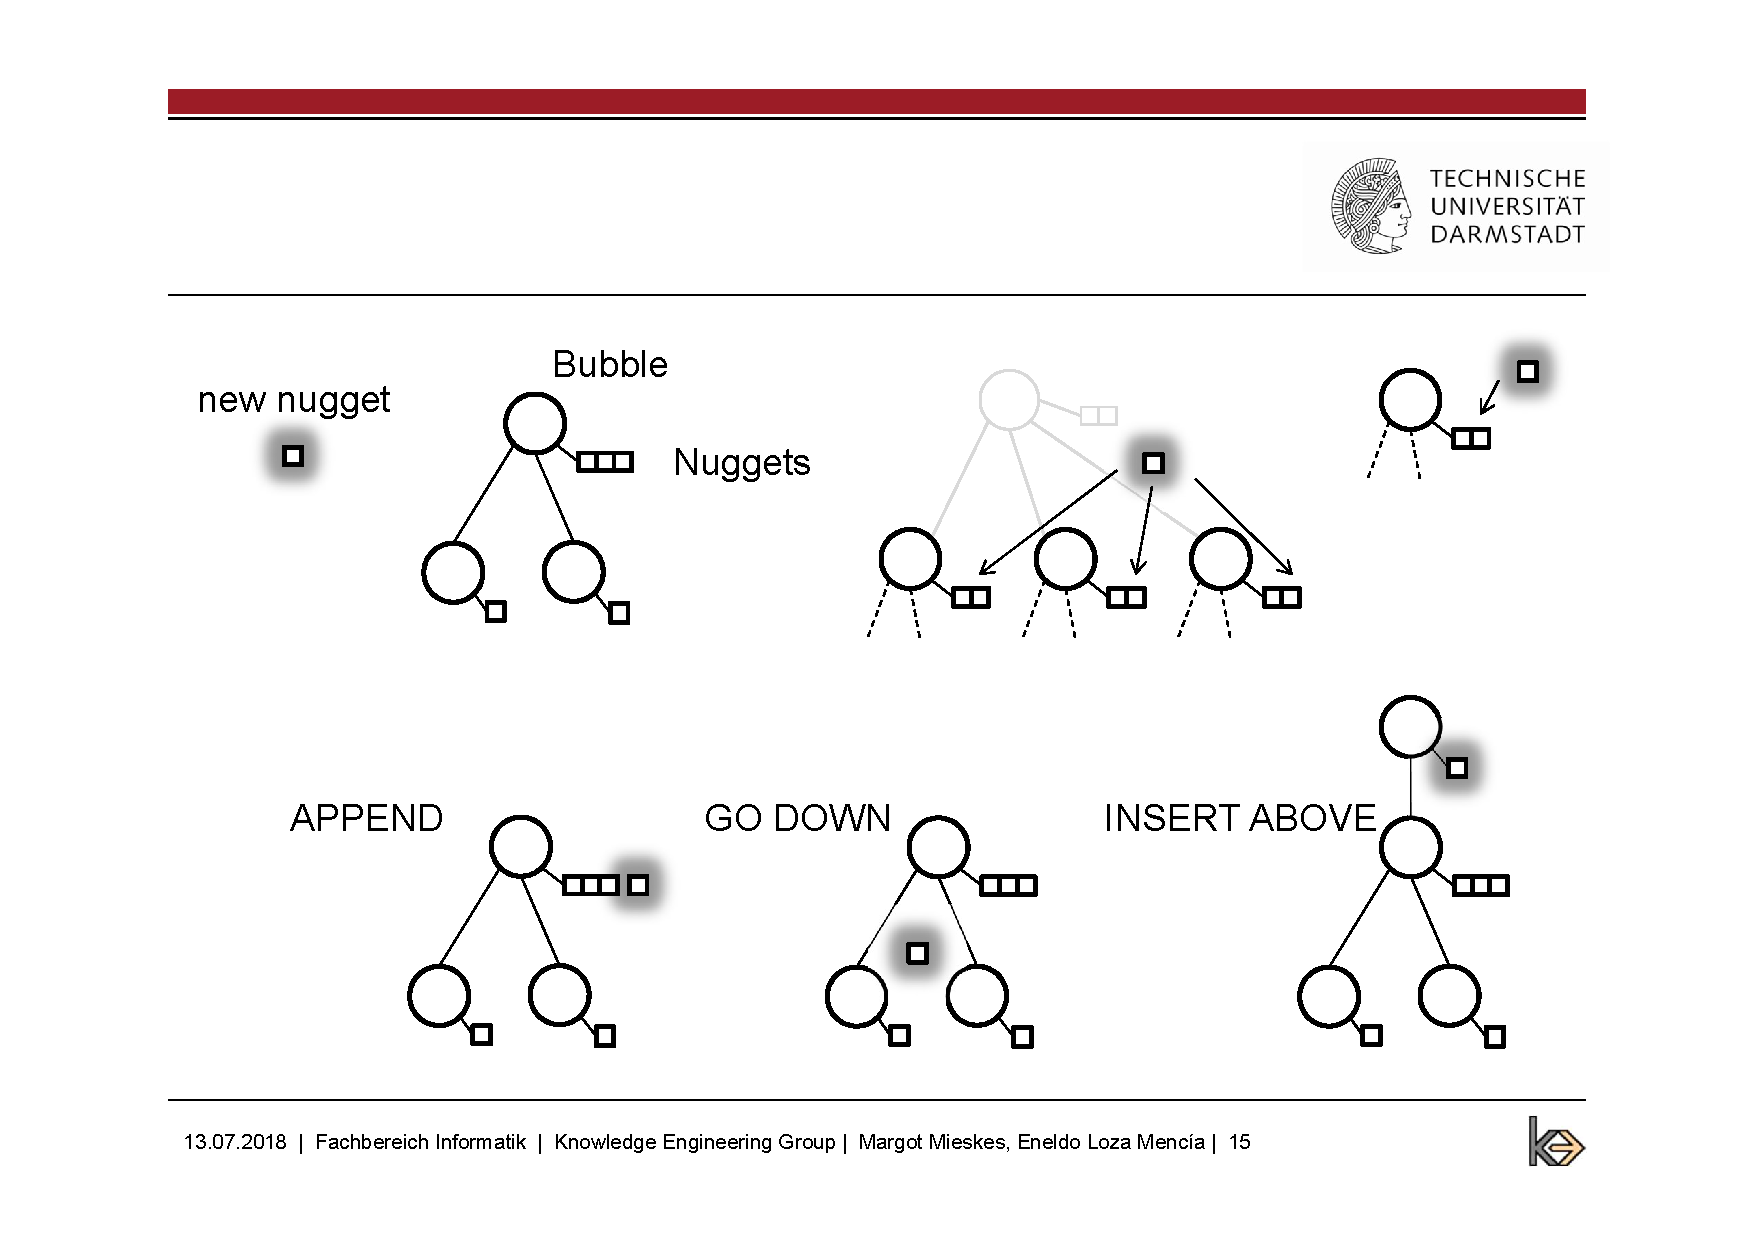
\includegraphics[trim=3cm 10cm 15cm 5.8cm, clip=true]{img/step2_func.pdf}
	\caption{new Nuggets and Bubble with Nugget}
	\label{fig:nuggetbubble}
\end{figure}
\subsubsubsection{\textbf{Insert function}}

The insert function takes a nugget and inserts it into the given tree. It runs recursively over the tree and calls the Which and Compare functions to determine where to go. Each step it first calls the Compare function which takes the current list of nuggets and the nugget which should be inserted. It returns the position where to insert the given nugget. There are three decicions to consider.
\begin{figure}[H]
	\centering
	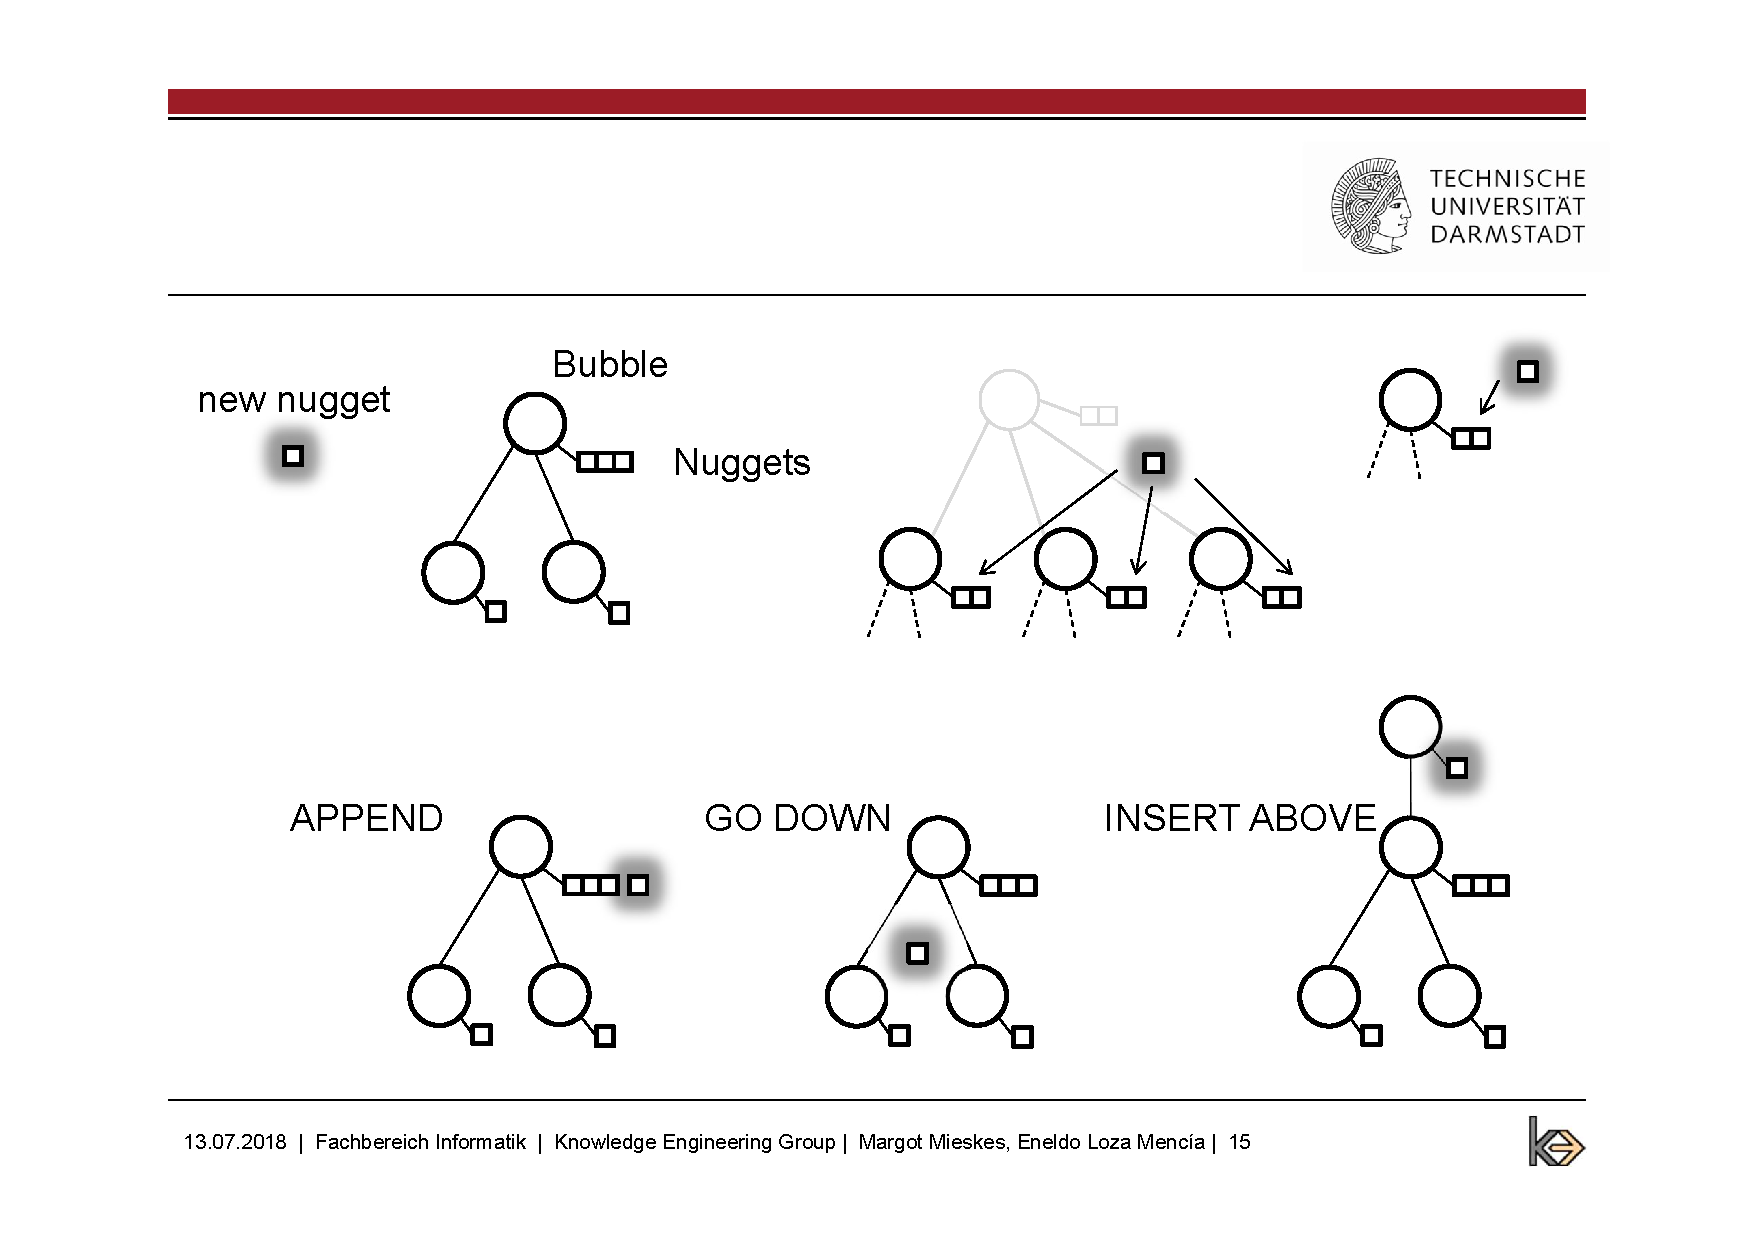
\includegraphics[trim=3.5cm 3cm 3cm 11cm, clip=true, width= \textwidth]{img/step2_func.pdf}
	\caption{Three results of Insert}
	\label{fig:insert}
\end{figure}

\begin{description}
\item [Append] It appends the given nugget to the current list of nuggets.
\item [Go Down] We call Which to determine in which bubble to go recursively. The which function returns the best Bubble to insert. The function then calls itself recursively in this Bubble.
\item [Insert Above] A new Bubble is created and inserted above the current Bubble and the pointers between the Bubbles are pointed to their new positions.
\end{description}

\subsubsubsection{\textbf{Which}}

The which function takes a list of Bubbles and the current Nugget to insert and returns the best position to insert the Nugget. This function tries to find the similarity of each Bubble to the current Nugget. Each Bubble can contain 1 to n Nuggets at the top level and multiple other in their siblings. We only take the 1 to n Nuggets in the top level and compare each word of each Nugget with NLTK path similarity.

% result = [[sim(x,y) for y in listb] for x in lista]
% flatten = [max(b) for b in result]
% value = reduce((lambda x, y: x + y), flatten) / len(flatten)

We calculate the similarity for each list of Nuggets of each Bubble against our given Nugget. This is done by calculating the path similarity for each word of the list of Nuggets against each word of the given Nugget. We take the maximal value for each word and then take the average of the list. We take the maximum of the list and compare it against a self-defined threshold value. The higher this threshold is the more new Bubbles are created and the lower the deeper the tree hierarchy is.

The NLTK path similarity returns a score that describes how similar two words are. The similarity is calculated by taking the shortest path that connects the senses of the words. The similarity value is in the range of 0 to 1.

\begin{figure}[H]
	\centering
	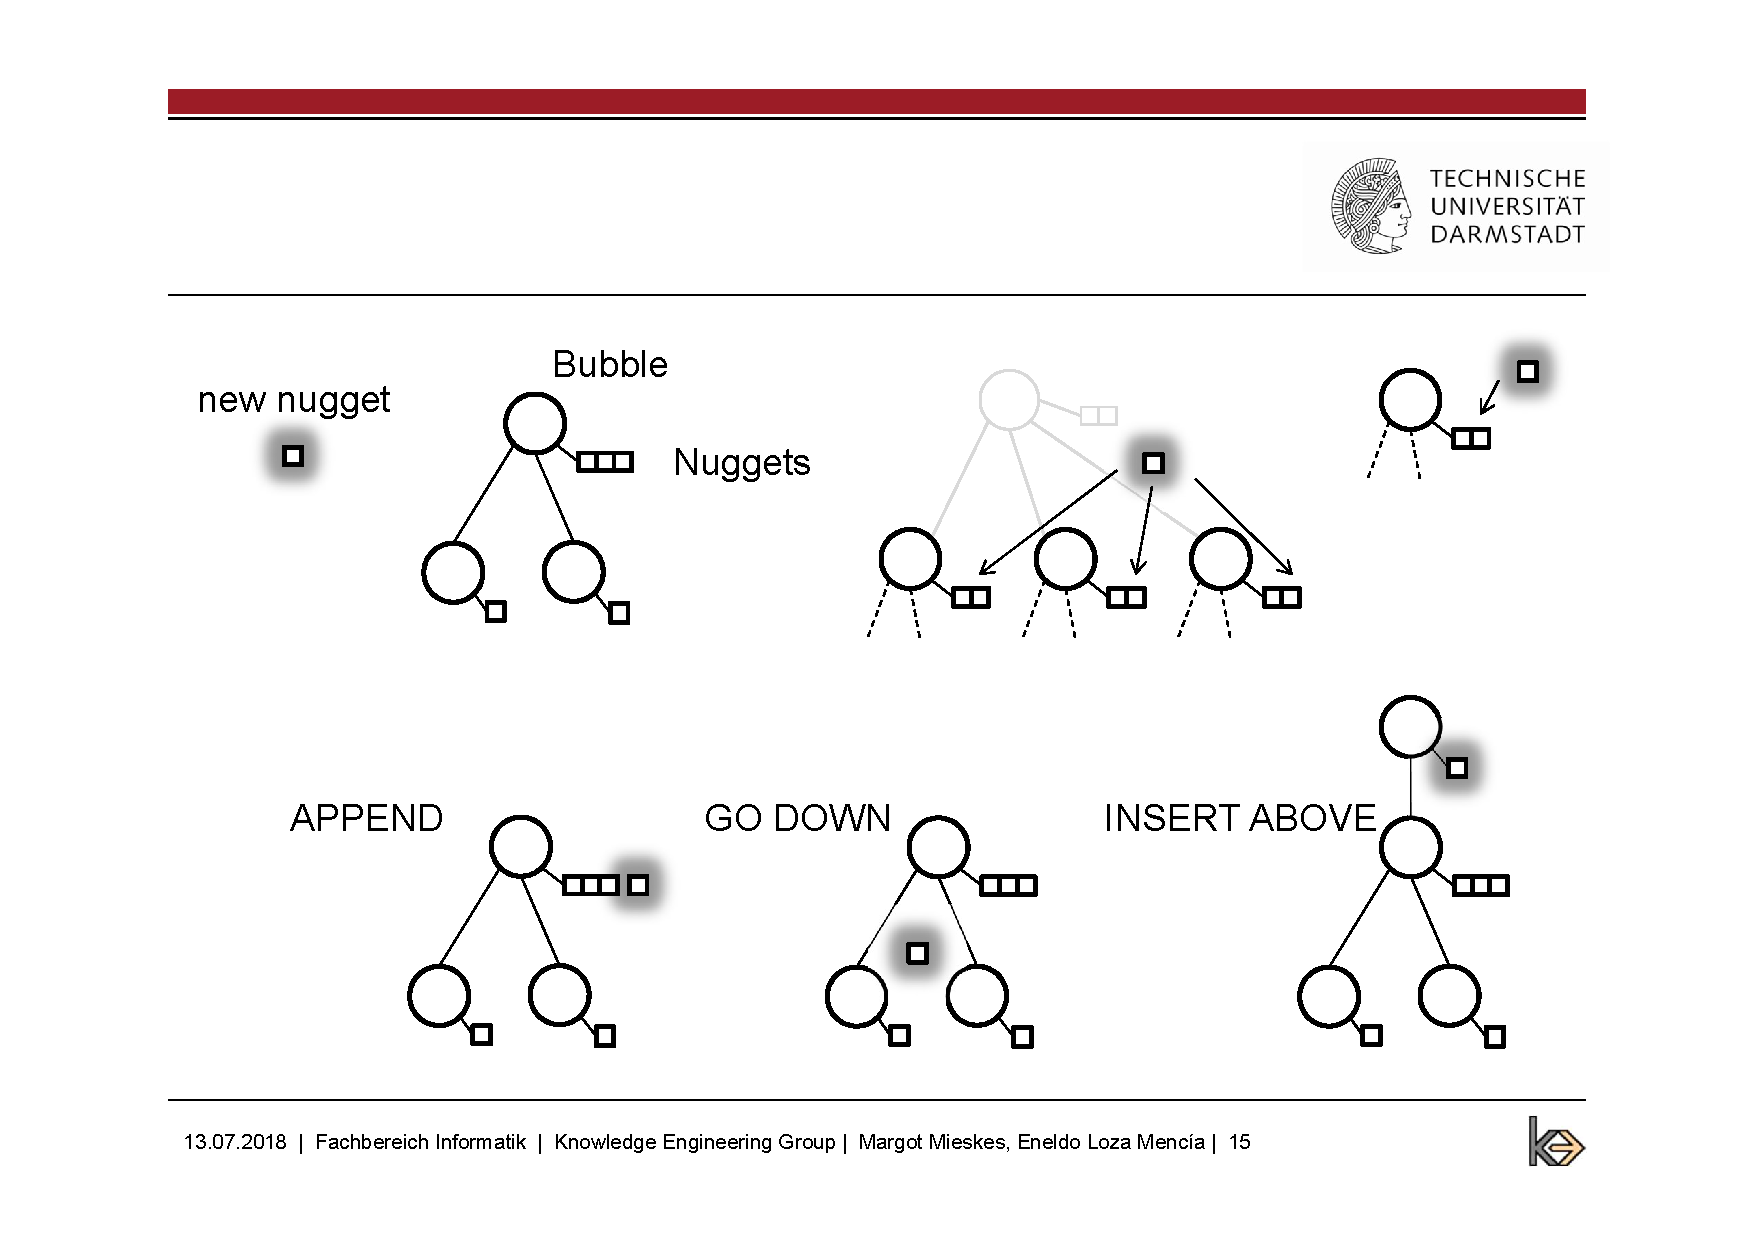
\includegraphics[trim=14cm 10cm 7cm 5.5cm, clip=true]{img/step2_func.pdf}
	\caption{Which Function}
	\label{fig:which}
\end{figure}


\subsubsubsection{\textbf{Compare}}

The compare function takes the current list of Nuggets and the Nugget which should be inserted and returns where to insert it (See List of decicions in Insert function). The goal of the compare function is to find which Nugget is more general or specific. We calculate the TF-IDF scores for the current nugget and the list of nuggets against the whole document. We do this because we want to find which Nugget is more important for the document.

TF-IDF is short for term frequency-inverse document frequency. The value increases by to the number of times a word appears in the document and is compensated by the frequency of the word in the document. This is done because some words appear more frequently in general. 


% sentenceList = sentence.GetWordsWithoutStopwords()
% sentenceResult = self.tfidf(sentenceList, self.table)
% nuggetsList2 = [self.tfidf(sublist.GetWordsWithoutStopwords(), self.table) for sublist in nuggets]
% nuggetsResult = reduce((lambda x,y: x+y), nuggetsList2) / len(nuggetsList2)


\begin{figure}[H]
	\centering
	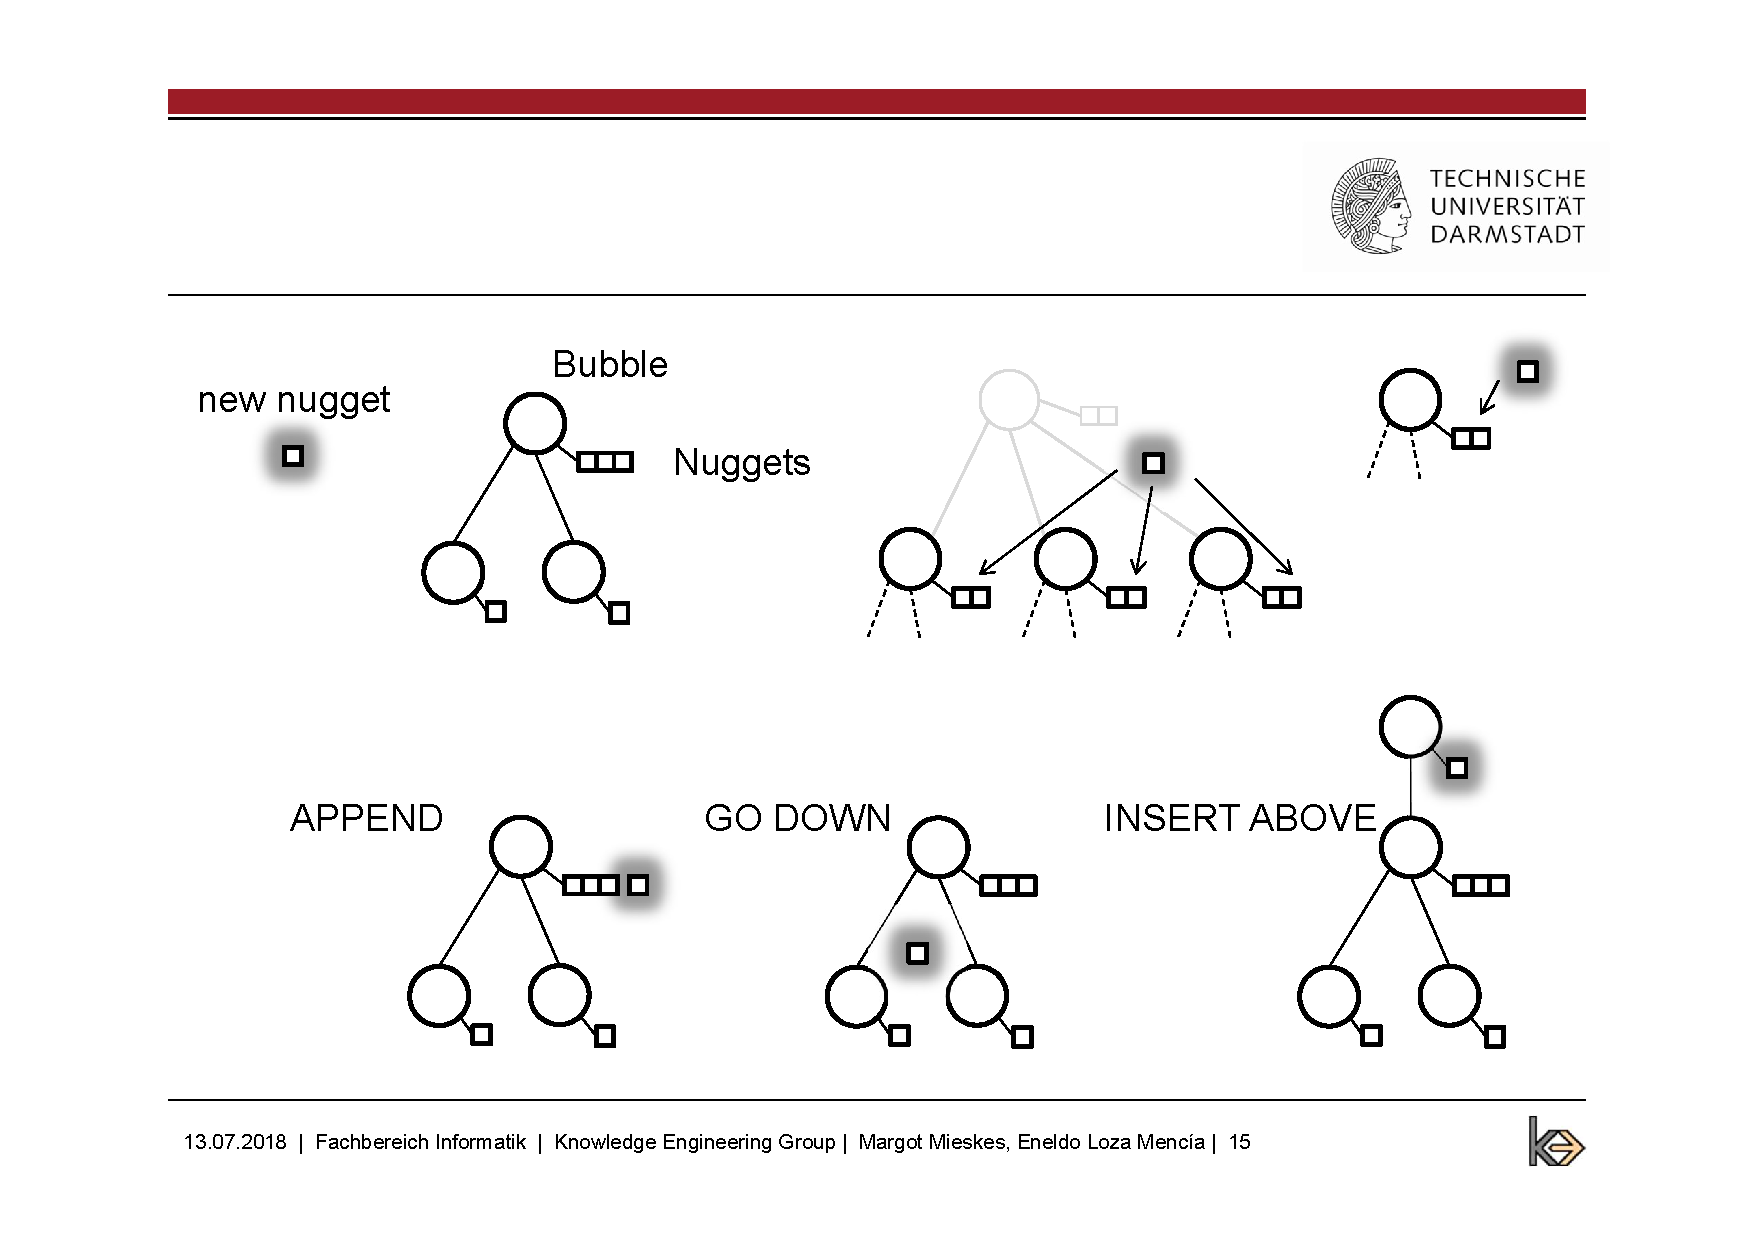
\includegraphics[trim=22.5cm 12.5cm 2.5cm 5.5cm, clip=true]{img/step2_func.pdf}
	\caption{Compare Function}
	\label{fig:compare}
\end{figure}


We thought about how we could improve our method and figured that an initial sorting of the Nuggets would help. This is already provided by the content selection of step 1. The best Nuggets appear at the beginning of the list. These Nuggets should be at the top of the hierarchy. We removed the Insert Above step from our insert function so that no Nuggets are inserted above. The Nuggets at the beginning of the list are now at the top of our hierarchy and the Nuggets further from the top are inserted deeper into the hierarchy. After we did this the quality of our resulting trees improved.

\subsubsection{Experimental Setup}

We used Python and NLTK.

\subsubsection{Experimental Results}

% https://github.com/AIPHES/HierarchicalSummarization

For the evaluation of the hierarchies, we used the \textit{Annotation Tool} from AIPHES \citep{Tauchmann.et.al.2018.LREC}. This tool was recommended in the lecture and can compare hierarchies against each other. It displays tree similarity of two given hierarchies and against random trees. It also shows network statistics such as the number of subtrees, subtree depth, average depth, total number of bubbles and average branching.

We first used the result of our method against the given gold standard. An issue was that our hierarchy only consists of 30 Nuggets instead of the 100 to 1400 Nuggets in the gold standard. We were not sure how this changes the result of the Annotation Tool. The results showed an average of 35 percent similarity. See figure \ref{fig:graph30} for the plotted similarity of the 10 topics.

\begin{figure}[H]
	\centering
	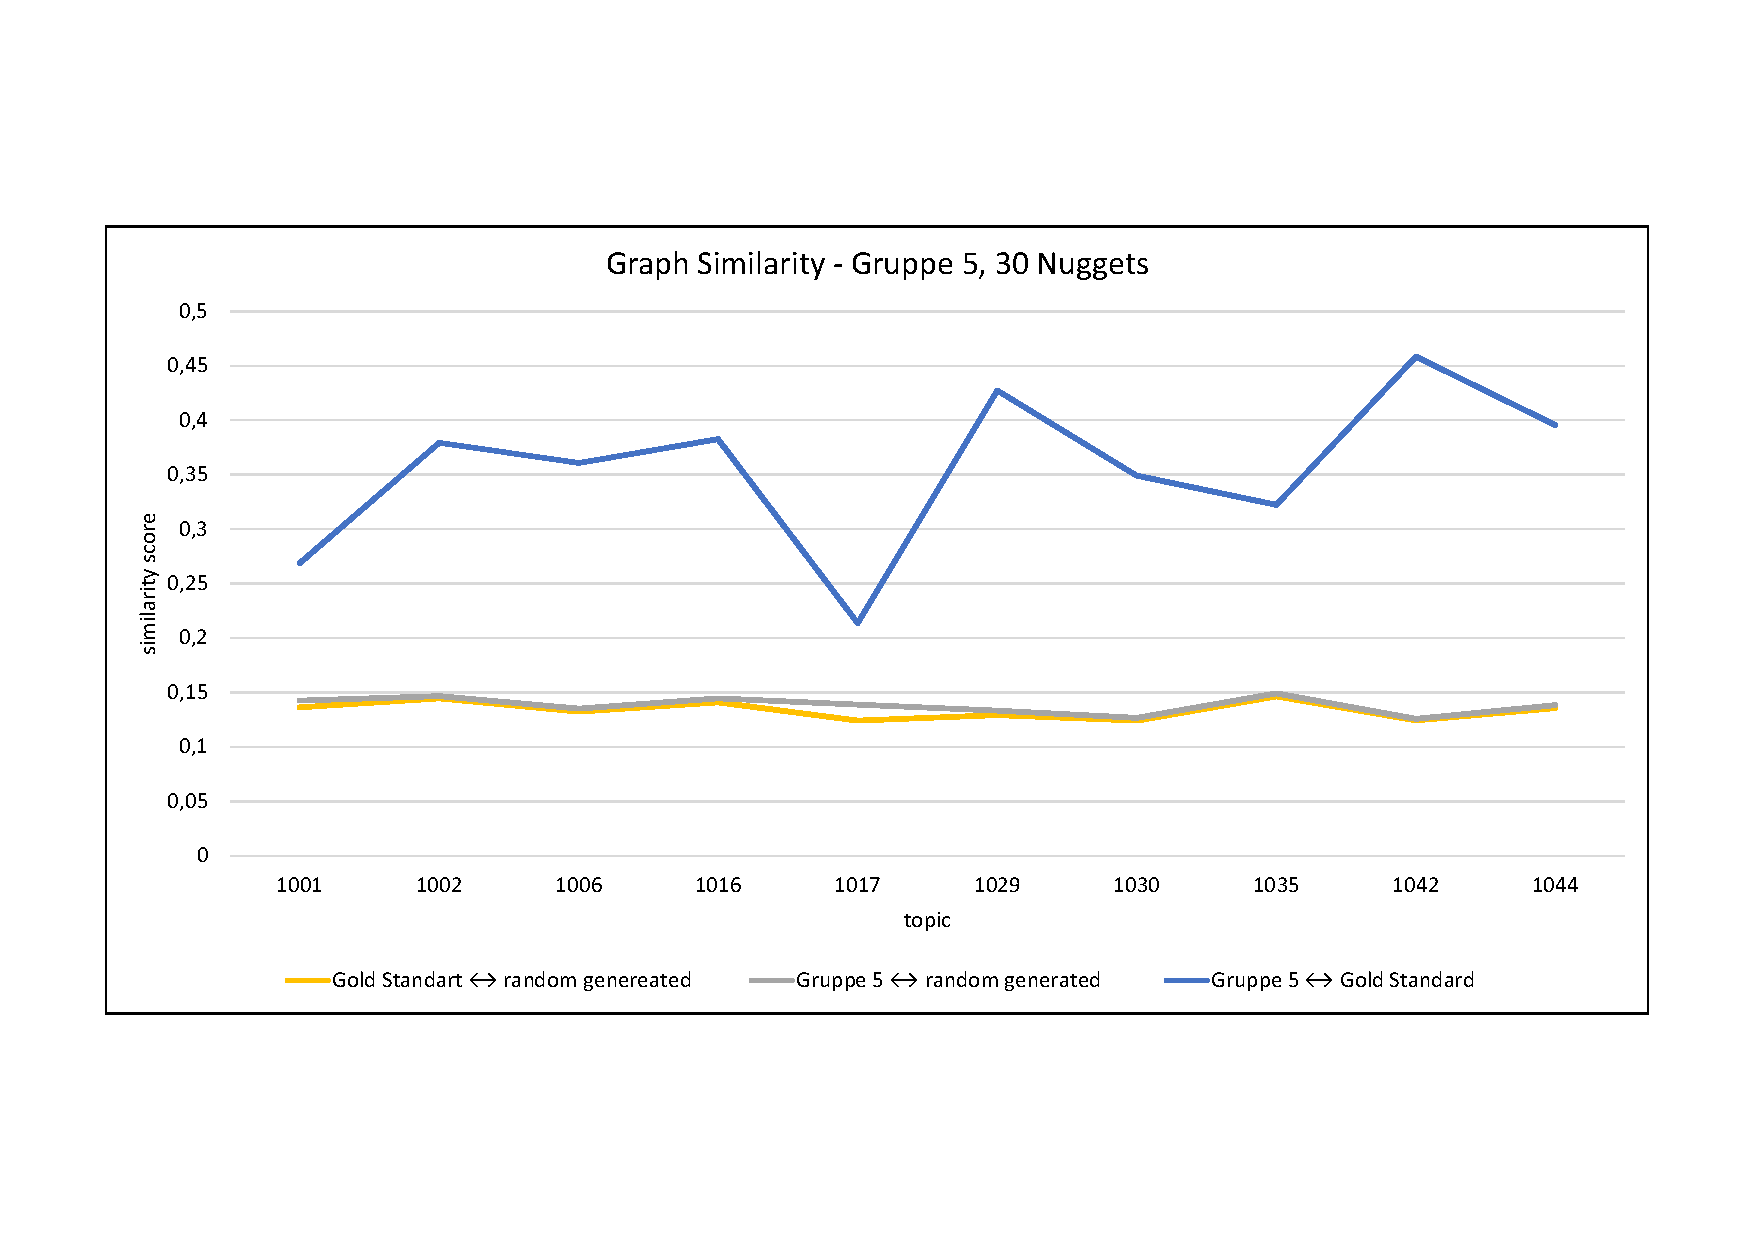
\includegraphics[trim= 0 130 0 130,width=\textwidth]{img/sim_v1.pdf}
	\caption{Graph Similarity with 30 Nuggets}
	\label{fig:graph30}
\end{figure}

We then ran our algorithm with all Nuggets to see how this changes the output of the \textit{Annotation Tool}. The issue here is that these Nuggets were not sorted by the content selection of our pipeline. The sorting of the Nuggets plays a major role in how our tree is built since we removed the Insert Above step.

The result can be seen in figure \ref{fig:graphn}. The similarity values of all three comparisons are very close. We concluded that the similarity is only noise and the trees differ too much.

Because our algorithm took a long time (up to 1 hour for one topic) for all Nuggets we could not use this evaluation intensively to improve our method. Instead, we tried to find a good balance for the number of Nuggets in each Bubble and the number of Bubbles in the root node. We applied a smoothing for the compare function to decrease the TF-IDF score when more Nuggets are present in the Bubble.

\begin{figure}[H]
	\centering
	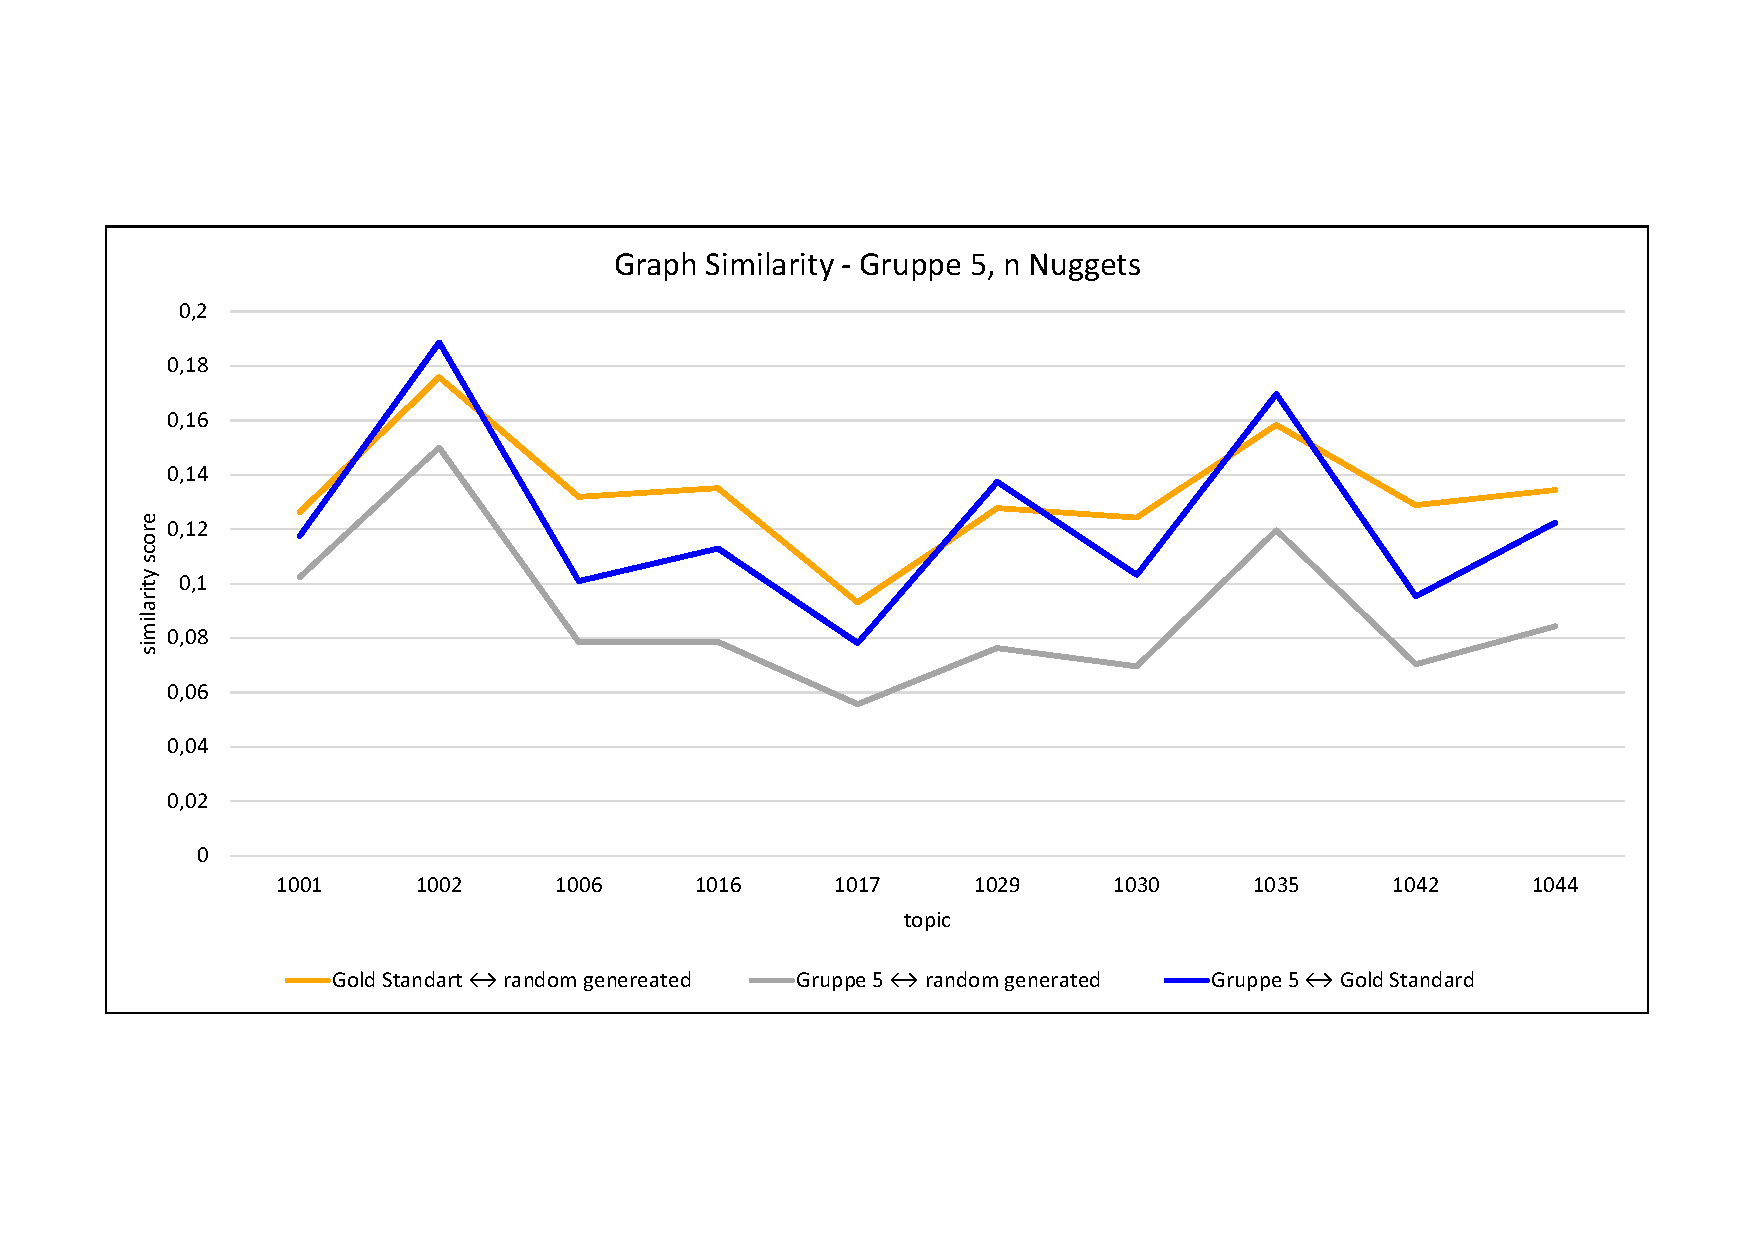
\includegraphics[trim= 0 130 0 130,width=\textwidth]{img/sim_v2.pdf}
	\caption{Graph Similarity with n Nuggets}
	\label{fig:graphn}
\end{figure}



\subsubsection{Discussion}

% hard to do an evaluation of performance on the system

% Is there a best (gold standard) hierarchy?
% Problem: How to define similarity of hierarchies?


This method can be easily improved by improving the two given functions which improve the overall system. For example, word embedding could be used to find similar Nuggets for the Which function. A clustering algorithm could be used to pre-sort the Nuggets into trees before inserting them. The compare function could be improved by using another term-weighting scheme or combining multiple.


% TODO: hard to define similar when we want general or specific

\subsubsection{Conclusions}

Our hierarchical ordering consists of three major parts. The recursive insert function, the Which function to determine where to insert a Nugget and the compare function to determine the position to insert the Nugget. We tested our method with the AIPHES \textit{Annotation Tool} and evaluated the results.


%\subsubsection{Bibliography}
% added at the end